\documentclass[a4paper,utf8]{article}
\usepackage{graphicx}
\usepackage[heading,fancyhdr]{ctex}
\usepackage{amsmath,amssymb,geometry,ulem}
\usepackage{array,tabularx,tabulary,mhchem,xspace}
\usepackage{floatrow,subfig,multirow,bigstrut}
\usepackage{siunitx,booktabs,longtable,nameref}
\lineskiplimit=1pt
\lineskip=3pt
\geometry{
    top=25.4mm, 
    left=25mm, 
    right=25mm, 
    bottom=25mm,
    headsep=5.9mm,
}
\ctexset{
    chapter = {
        name = {实验,},
        beforeskip = {-23pt}
    }
}
\newcommand{\fgref}[1]{图~\ref{#1}\xspace}
\newcommand{\seqref}[1]{式~(\ref{#1})}
\newcommand{\expinfo}[6][无]{
    {\zihao{-3}\bfseries\songti
    实验名称:\uline{\hfill\mbox{#2}\hfill} \\[2.9mm]
    学\quad 号:\uline{\makebox[25mm]{#3}}\hfill
    姓\quad 名:\uline{\makebox[25mm]{#4}}\hfill
    班\quad 级:\uline{\makebox[25mm]{#5}} \\[2.9mm]
    合作者:\uline{\makebox[25mm]{#1}} \hfill
    桌\quad 号:\uline{\makebox[25mm]{}}\hfill\makebox[25mm+4em]{}\\[2.9mm]
    指导教师:\uline{\makebox[30mm]{#6}}\hfill\mbox{} \\[2.9mm]
    实验日期:\uline{\makebox[30mm]{}}\hfill\mbox{} \\[58.7mm]
    }
}%\expinfo[合作者]{实验名称}{学号}{姓名}{班级}{指导教师}
\newcommand{\pointingbox}{
    {\zihao{4}\bfseries\songti%
    实验考核\\[3mm]
    \extrarowheight=3mm
    \begin{tabularx}{150mm}{|X|X|X|X|X|}\hline
        \hfil 项目 \hfil  & \hfil 实验预习 \hfil & \hfil 实验过程 \hfil & \hfil 分析与讨论 \hfil & \hfil 总评 \hfil \\[3mm] \hline
        \hfil 评价 \hfil &  &  &  &  \\[3mm] \hline
    \end{tabularx}
    }
}
\newcommand{\derivative}[2]{\frac{\mathrm{d} #1}{\mathrm{d} #2}}
\newcommand{\thinking}[2]{\textbf{#1}\\
答:\begin{minipage}[t]{0.85\textwidth}
    #2
\end{minipage}}

\pagestyle{fancy}
\fancyhf{}
%\fancyhead[C]{材料科学基础实验}
%\fancyfoot[C]{\thepage}
\fancyhead[EC]{\leftmark} \fancyhead[OC]{\rightmark}
\fancyhead[EL,OR]{\thepage}
\fancypagestyle{plain}{\renewcommand{\headrulewidth}{0pt}\fancyhf{}}

\newcounter{Rownumber}
\newcommand*{\Rown}{\stepcounter{Rownumber}\theRownumber}
\newcounter{sample}
\newcommand*{\Sam}{\stepcounter{sample}\thesample}
\newcounter{Fignumber}
\newcommand*{\Fign}{\stepcounter{Fignumber}\theFignumber}

\newcommand*{\resetRown}{\setcounter{Rownumber}{0}}
\newcommand{\qrange}[3]{\qtyrange[range-phrase = \text{$\sim$},range-units =single]{#1}{#2}{#3}}
\floatsetup[table]{capposition=top}
\newcolumntype{C}{>{\hfil}X<{\hfil}}
\renewcommand{\Nameref}[1]{\textbf{\ref{#1}~\nameref{#1}}}
\newcommand{\TTR}[0]{\watt\per\m\per\K}
\newcommand{\TTR}[0]{\watt\per\m\per\K}
\begin{document}
\begin{center}
    {\mbox{}\\[7em]\zihao{2}\bfseries\songti%
    材料科学基础实验报告}\\[34mm]
    \expinfo{使用热流计法和平面热源法测量材料的热导率}{22301077}{张蕴东}{22高分子}{艾斌}
    {\zihao{4}\bfseries\songti
    实验考核\\[3mm]
    \extrarowheight=3mm
    \begin{tabularx}{150mm}{|X|X|X|X|X|}\hline
        \hfil 项目 \hfil  & \hfil 实验预习 \hfil & \hfil 实验过程 \hfil & \hfil 分析与讨论 \hfil & \hfil 总评 \hfil \\[3mm] \hline
        \hfil 评价 \hfil &  &  &  &  \\[3mm] \hline
    \end{tabularx}
    }
\end{center}\newpage
\newpage
\section{实验目的}
    \begin{itemize}
        \item 了解稳态热流计法测量材料的热导率(或导热系数)和样品的热阻的原理;
        \item 学会使用稳态热流计法测量不同材料的热导率和样品的热阻;
        \item 了解准稳态平面热源法测量材料的热导率和比热的原理;
        \item 学会用准稳态平面热源法测量材料的热导率和比热。
    \end{itemize}
\section{实验原理}%简单描述,含必要的公式和附图;
    \subsection{热传导理论中的一些基本概念}
        傅立叶热传导定律指出,通过材料的热传导速率(单位时间传递的热量)与温度的梯度和热量流经的横截面积成正比。对于均匀介质中的一维热传导,傅立叶热传导定律可以表示为:
        \begin{equation}
            q_c=-kA\frac{dT}{dx}\label{eq:1}
        \end{equation}\par
        材料的热导率 $k$(或导热系数)可理解为单位温度梯度下、单位时间内通过单位横截面积的热量。热导率是表征材料热学性能的一个重要参数,不同的材料具有不同的热导率,譬如 Cu 的热导率为 399 \unit{\TTR},玻璃的热导率为 0.81 \unit{\TTR},塑料的热导率为 \qrange{0.2}{0.3}{\TTR},而空气的热导率仅为 0.026 \unit{\TTR}。负号表示热量总是从温度高的位置流向温度低的位置。需要说明的是,傅立叶定律适用于一维稳态热传导问题。根据\seqref{eq:1},材料的热导率可写作:
        \begin{equation}
            k=\frac{q_c}{A \displaystyle \left|\frac{dT}{dx}\right|} \label{eq:2}
        \end{equation} \par
        为了引入热阻的概念,已知一块长方体匀质材料左侧的温度为 $T_1$,右侧的温度为 $T_2$,且 $T_1 > T_2$,两个侧面相距 $L$,热传导的横截面积为 $A$,假设单位时间从左侧传递到右侧的热量(即热传导的速率)为$q_c$,则材料的热阻为:
        \begin{equation}
            R_t=\frac{T_1-T_2}{q_c}=\frac{1}{k}\cdot\frac{L}{A} \label{eq:3}
        \end{equation} \par
    \subsection{测量材料热导率的方法简介}
        有多种测量材料热导率的方法,这些方法大致可分为两类:稳态法和瞬态法。稳态法是在样品处于稳态热传导的条件下(样品内部的温度分布不随时间变化)进行测量的方法。稳态法包括保护平板法(测量范围 \qrange{0.001}{2}{\TTR})、热流计法(测量范围 \qrange{0.001}{20}{\TTR})和保护热流计法(测量范围 \qrange{0.01}{400}{\TTR})。稳态法的优点是利用傅立叶热传导定律计算热导率,计算过程简单,缺点是要求材料达到稳定热传导的状态,测试时间长等。瞬态测量方法是在样品处于非稳态热传导条件下进行测量的方法。瞬态法包括热线法(测量范围 \qrange{0.01}{20}{\TTR})、瞬态平面热源法(测量范围 \qrange{0.01}{20}{\TTR})和激光闪光法(测量范围 \qrange{0.1}{2000}{\TTR})。准稳态法的优点是测量速度快、测量范围宽,缺点是设备较为复杂和昂贵。
        \subsubsection{热流计法测量材料热导率的原理}
            \fgref{fg:1} 给出了热流计法测量材料热导率的原理示意图。如图所示,加热面 A 将热量经待测样品 B 传导到散热面 C(室温)。由于加热面 A 和散热面 C 都是由热的良导体铜板制作,且与待测样品 B 紧密接触,当达到稳态时可认为其温度就是样品上、下表面的温度 $T_1$ 和 $T_2$,且 $T_1 > T_2$。对于样品 B,假设其导热方向的厚度为 $L$,面积为 $A$,当达到稳态热传导时,只要准确测量出样品的厚度 $L$ 和面积 $A$、上下表面的温度 $T_1$和 $T_2$,以及流经样品的热流 $q_c$,就可以利用\seqref{eq:3}计算材料的热导率和热阻。
            \begin{figure}[!ht]\centering
                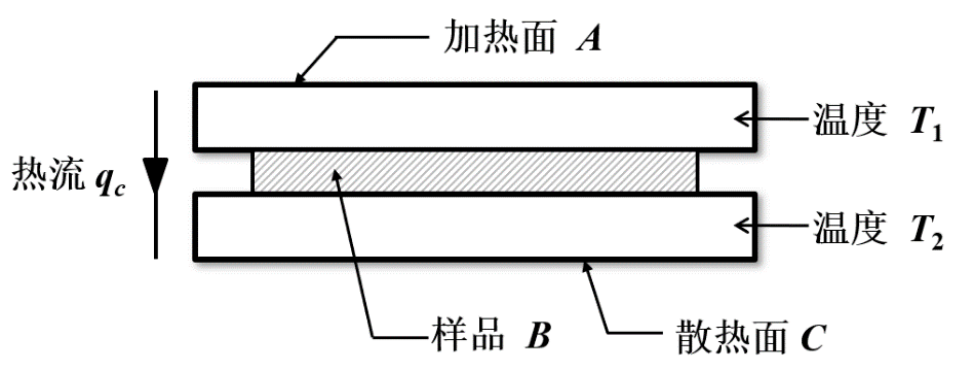
\includegraphics[width=100mm]{fg1.png}
                \caption{热流计法测量材料热导率的原理示意图 \label{fg:1}}
            \end{figure}
        \subsubsection{平面热源法测量材料热导率的原理}
            如\fgref{fg:2}所示,考虑一无穷大导热平板的一维热传导问题。假设该平板的面积为无限大、厚度为 $2d$,初始温度为 $T_0$。现从平板的两侧同时向中心面施加均匀的热流密度(单位时间通过单位截面积的热量,也被称为热通量)$q_f$(\unit{\watt\per\meter\squared}),则平板上各点的温度 $T(x,t)$ 将随加热时间 $t$而变化。
            \begin{figure}[!ht]\centering
                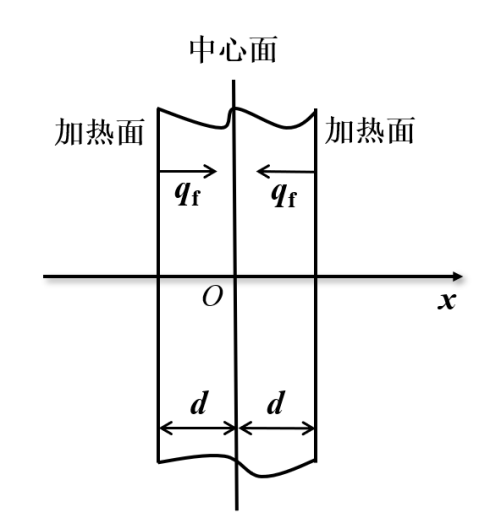
\includegraphics[width=50mm]{fg2.png}
                \caption{厚度为 $2d$ 的无穷大导热平板的一维热传导模型示意图 \label{fg:2}}
            \end{figure}\par
            以样品中心面上的一点为坐标原点 $O$,以样品厚度方向为 $x$ 轴方向,如\fgref{fg:2} 所示,则平板上各处的温度$T(x,t)$随位置 $x$和加热时间 $t$的分布可通过求解下面的偏微分方程得到:
            \begin{equation}
                \begin{cases}
                    \frac{\partial T(x,t)}{\partial t}=\alpha\frac{\partial^2T(x,t)}{\partial x^2}\\
                    \frac{\partial T(d,t)}{\partial x}=\frac{q_f}k ,\quad\frac{\partial T(0,t)}{\partial x}=0\\
                    T(x,0)=T_0
                \end{cases}
            \end{equation}
            该偏微分方程的解说明了当热流密度$q_c$恒定时,此时加热面和中心面之间的温度差$\varDelta T$保持恒定,与加热时间 $t$ 无关,我们称这种状态为准稳态。当体系到达准稳态时:\par
            \begin{equation}
                \begin{aligned}
                    k&=\frac{q_fd}{2\Delta T}\\
                    c&=\frac{q_f}{\rho d\frac{\partial T}{\partial t}}
                \end{aligned}
            \end{equation}
\section{实验仪器}%规格及参数
    DRPL-I热导率测试仪,计算机,ZKY-BRDR 型准稳态法热导率、比热测试仪,样品(石英、白橡胶、铝合金、黑橡胶、有机玻璃)。
\section{实验过程}%简述主要过程和实验内容
    \subsection{使用稳态法(热流计法)测量样品的热阻和材料的热导率}
        本实验使用 ZKY-BRDR 型热导率测试仪和基于瞬态测试方法的平面热源法对两种样品(黑橡胶和有机玻璃)的热导率和比热进行测试。给出了 ZKY-BRDR 型准稳态法热导率、比热测试仪的正面照片。如图所示,该测试仪由主机、卧式测试装置和保温杯三部分组成。主机的前面板有电源开关、加热电压调节旋钮、加热电压/热电势切换开关、中心面/温差热电势切换开关、加热电压/热电势显示、加热计时显示、加热计时清零按钮、加热指示灯。需要说明的是,加热开关位于主机的后面板上。一旦打开加热开关,加热指示灯就会点亮,加热计时就会显示加热时间。实验人员可通过操作主机上的相关开关或旋钮,人工完成所有实验数据的采集。卧式测试装置用来固定和压紧样品、对样品加热和测温、并将热电偶输出的温差热电势信号放大后输入到测试主机上。保温杯的作用是使两个热电偶的冷端在整个实验过程中保持温度恒定。
        \subsubsection{测量方块状白橡胶样品的热阻和白橡胶的热导率}
        \subsubsection{测量圆柱形石英样品的热阻和石英的热导率}
        \subsubsection{测量圆柱形铝合金样品的热阻和铝合金的热导率}
    \subsection{使用准稳态法(平面热源法)测量有机玻璃和黑橡胶的热导率和比热}
        要使用 ZKY-BRDR 型测试仪测量材料的热导率和比热,需准备 4 块尺寸完全相同的同质样品。四块样品 1、2、3 和 4 一字排开,样品 2 和 3 之间的中央位置放置中心面热电偶测温端;样品 1 和 2 之间为面加热器1,样品 3 和 4 之间为面加热器 2,并在样品 3 和面加热器 2 之间的中央位置放置加热面热电偶测温端。测试时,四块样品和两个面加热器被紧密挤压在一起,确保样品和样品之间以及样品和加热器之间不存在空气隙,且样品和加热器周围被绝热材料所包围。由于面加热器可对整个样品面积进行均匀加热,且样品的横向尺寸大于样品厚度的 6 倍以上,可以认为热传导只沿样品厚度方向进行,所以之前在假设样品为无穷大的前提下推导出来的一维非稳态热传导公式对本实验仍然近似成立。由于面加热器可以向左、右两边加热,所以在每个面加热器的两边配置了两个相同的样品(它们具有相同的热阻),这样可使样品 2 或 3 获得的热流密度约等于面加热器一半的电功率。一旦确定了样品 2 和 3 从面加热器获得的热流密度 $q_f$ ,只需测出体系进入准稳态后加热面和中心面之间的温度差(或样品 3 两侧的温度差)$\delta T$,就可以计算材料的热导率。由于我们在样品 3 的两侧分别放置了中心面热电偶的测温端和加热面热电偶的测温端,且两个热电偶的冷端被放置在同一个保温杯中,在整个实验过程中两个热电偶的冷端温度保持恒定,所以测试过程中任意时刻样品 3 两侧的温差热电势 $V_t$(即两个热电偶的测温端温差热电势)可以由仪器测出。自然,我们便可以计算出材料的比热。
        \subsubsection{测量有机玻璃的热导率和比热}
        \subsubsection{测量黑橡胶的热导率和比热}
\section{实验结果}
    \subsection{使用稳态法测量圆柱形铝合金样品的热阻和热导率}
        报告结果随附,以下是误差分析:\par
        已知温度测量范围为: \qrange{19}{99.99}{\degreeCelsius},温度测量精度 $\pm 0.05 \unit{\degreeCelsius}$ 。热流计热流测量范围:\linebreak \qrange{0.5}{2000}{\watt},分辨率 0.25 \unit{\watt} 。游标卡尺的测量精度为 0.02 \unit{\mm} 。假定矩形分布来评估仪器精度引入的不确定度。计算样品热导率测量结果的相对不确定度。假设包含因子 $k=2$,给出扩展不确定度。
        \begin{figure}[!ht]
            \subfloat[MMA 计算不确定度的源代码]{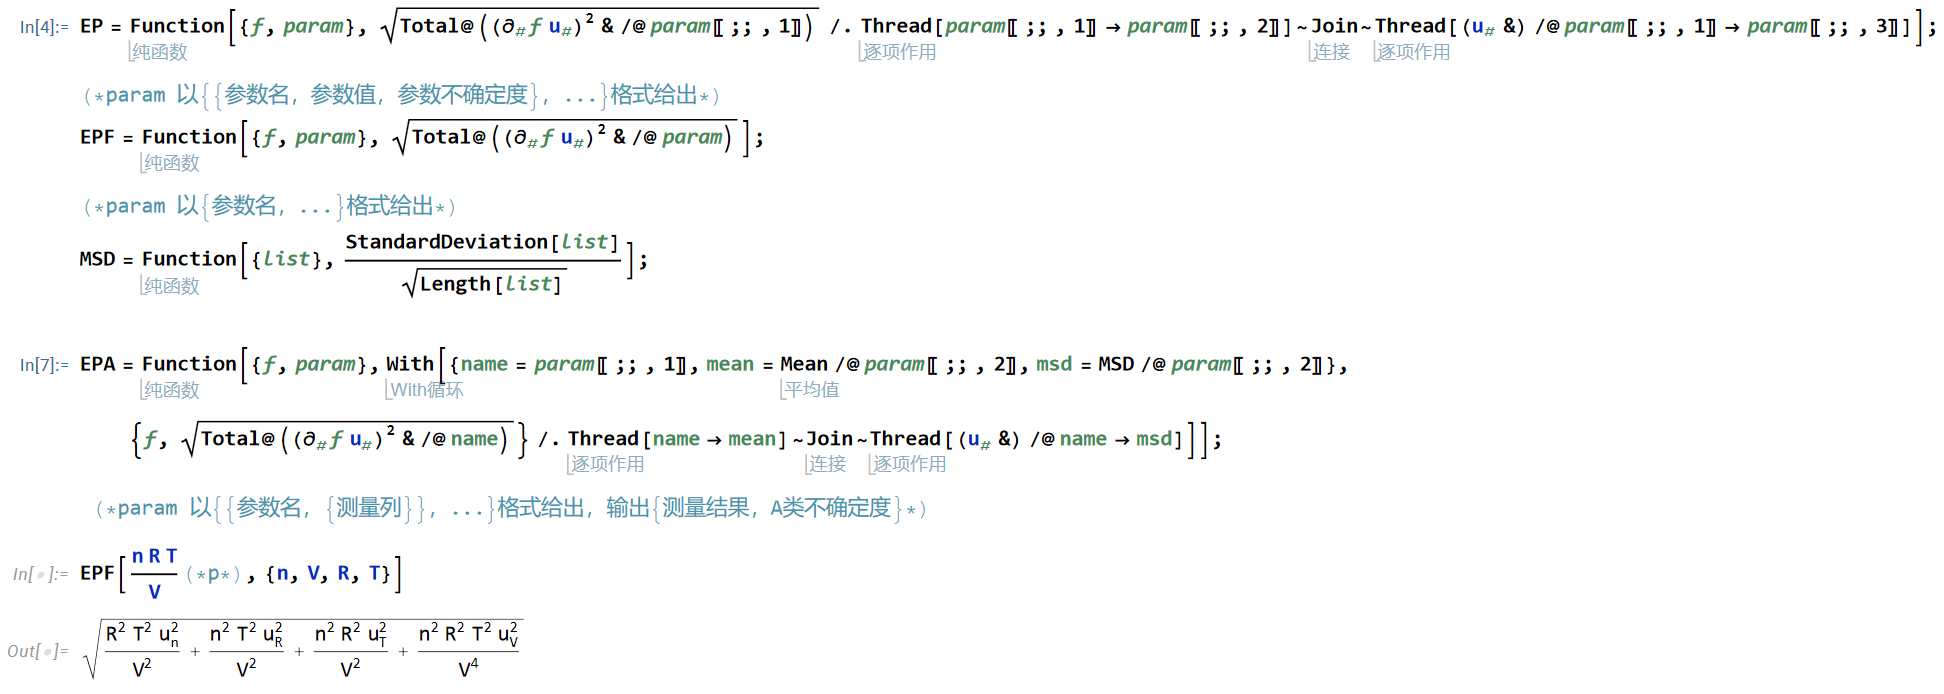
\includegraphics[width=\textwidth]{EF.png}}\par
            \subfloat[使用 MMA 计算不确定度]{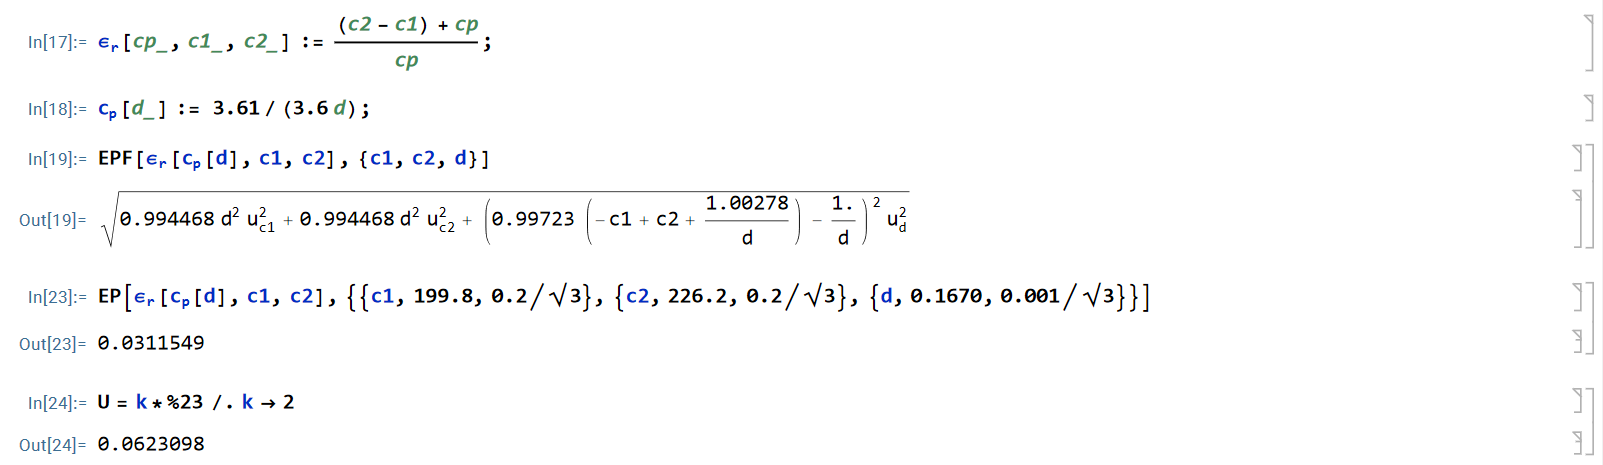
\includegraphics[width=\textwidth]{result.png}}
        \end{figure}\par
        最后得到的拓展不确定度为:
        \begin{equation*}
            k = ( 121.44 \pm 0.27 ) \unit{\TTR}
        \end{equation*}
        其中在“$\pm$”号后的数为扩展不确定度 $U=ku_c$ 的数值, $ U $ 是由 $ u_c= 0.139251 \unit{\ohm\cm}$ 和 $ k = 2 $ 确定的, $k$ 是基于矩形分布得到的,自由度在讲义中未提到。确定区间的包含概率在讲义中未提到。\newpage
    \subsection{由Origin处理后绘制的图像}
        \begin{figure}[!ht]
            \subfloat[有机玻璃]{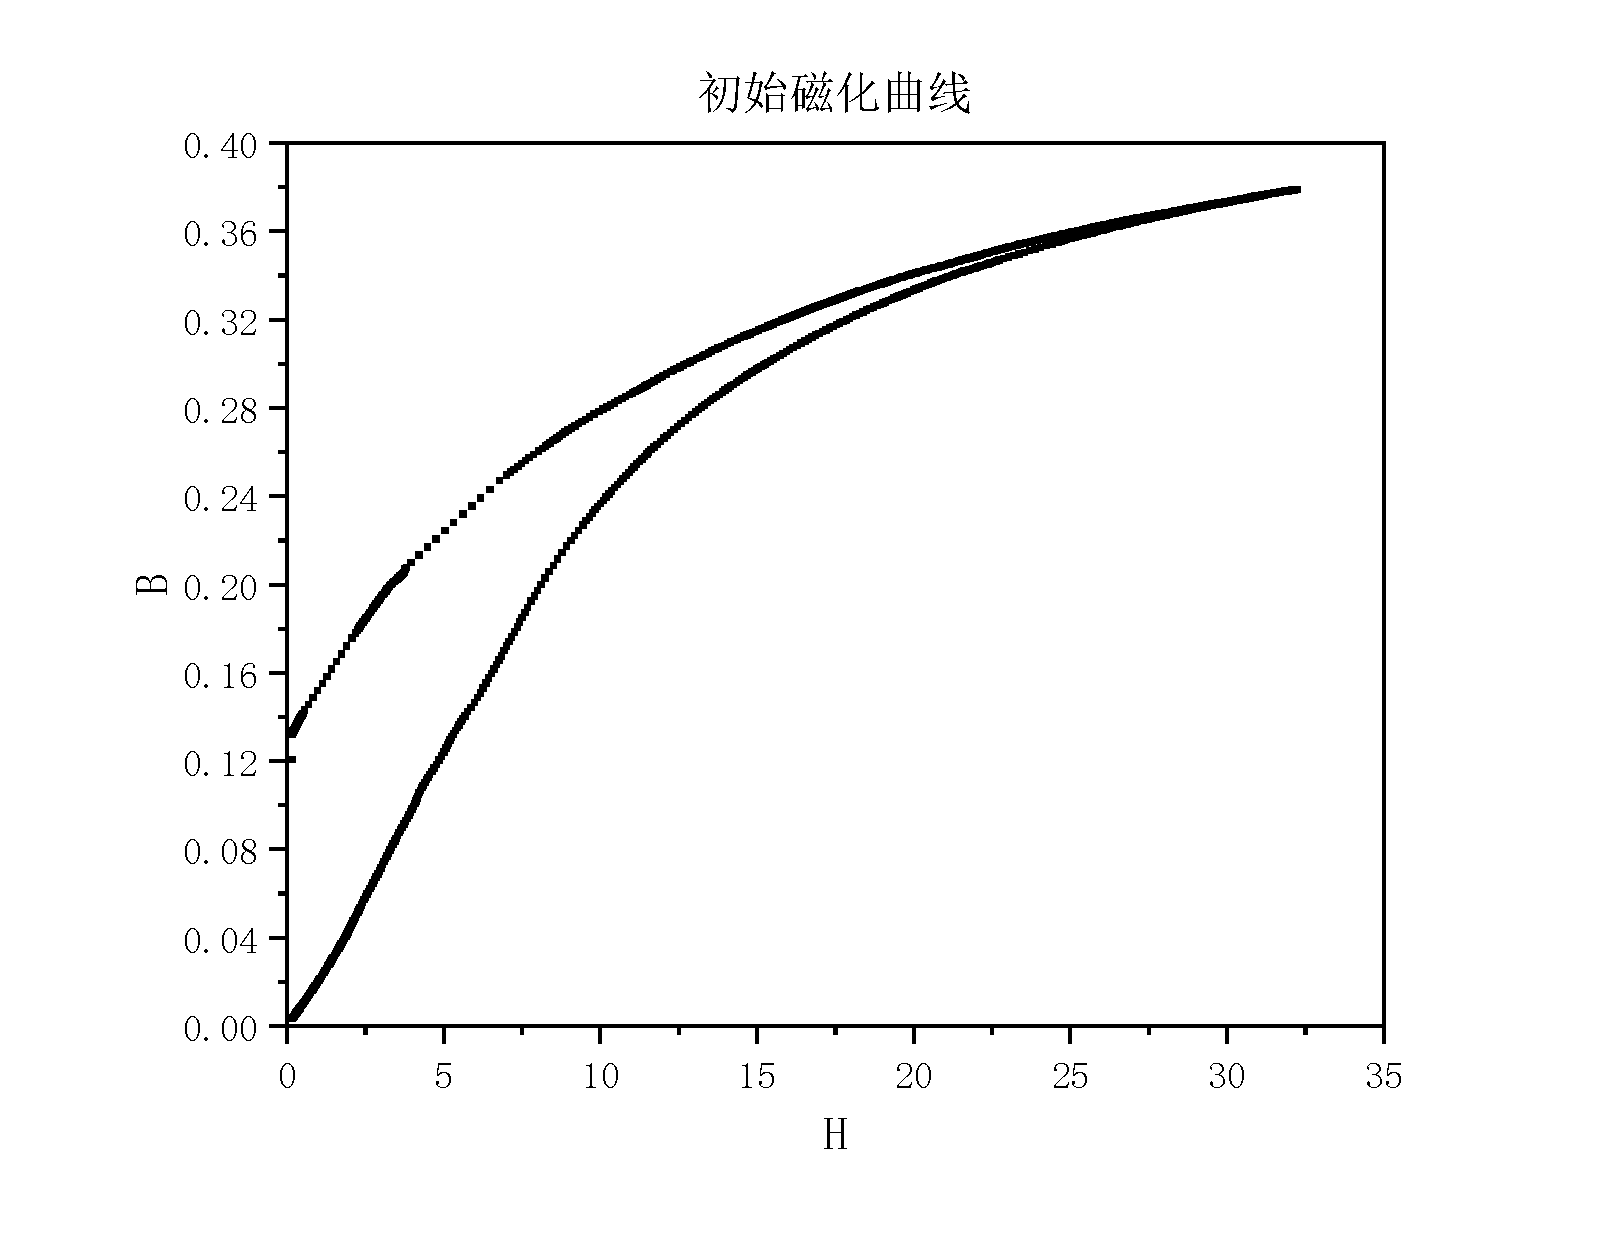
\includegraphics[width=0.8\textwidth]{fig2.pdf}}\par
            \subfloat[黑橡胶]{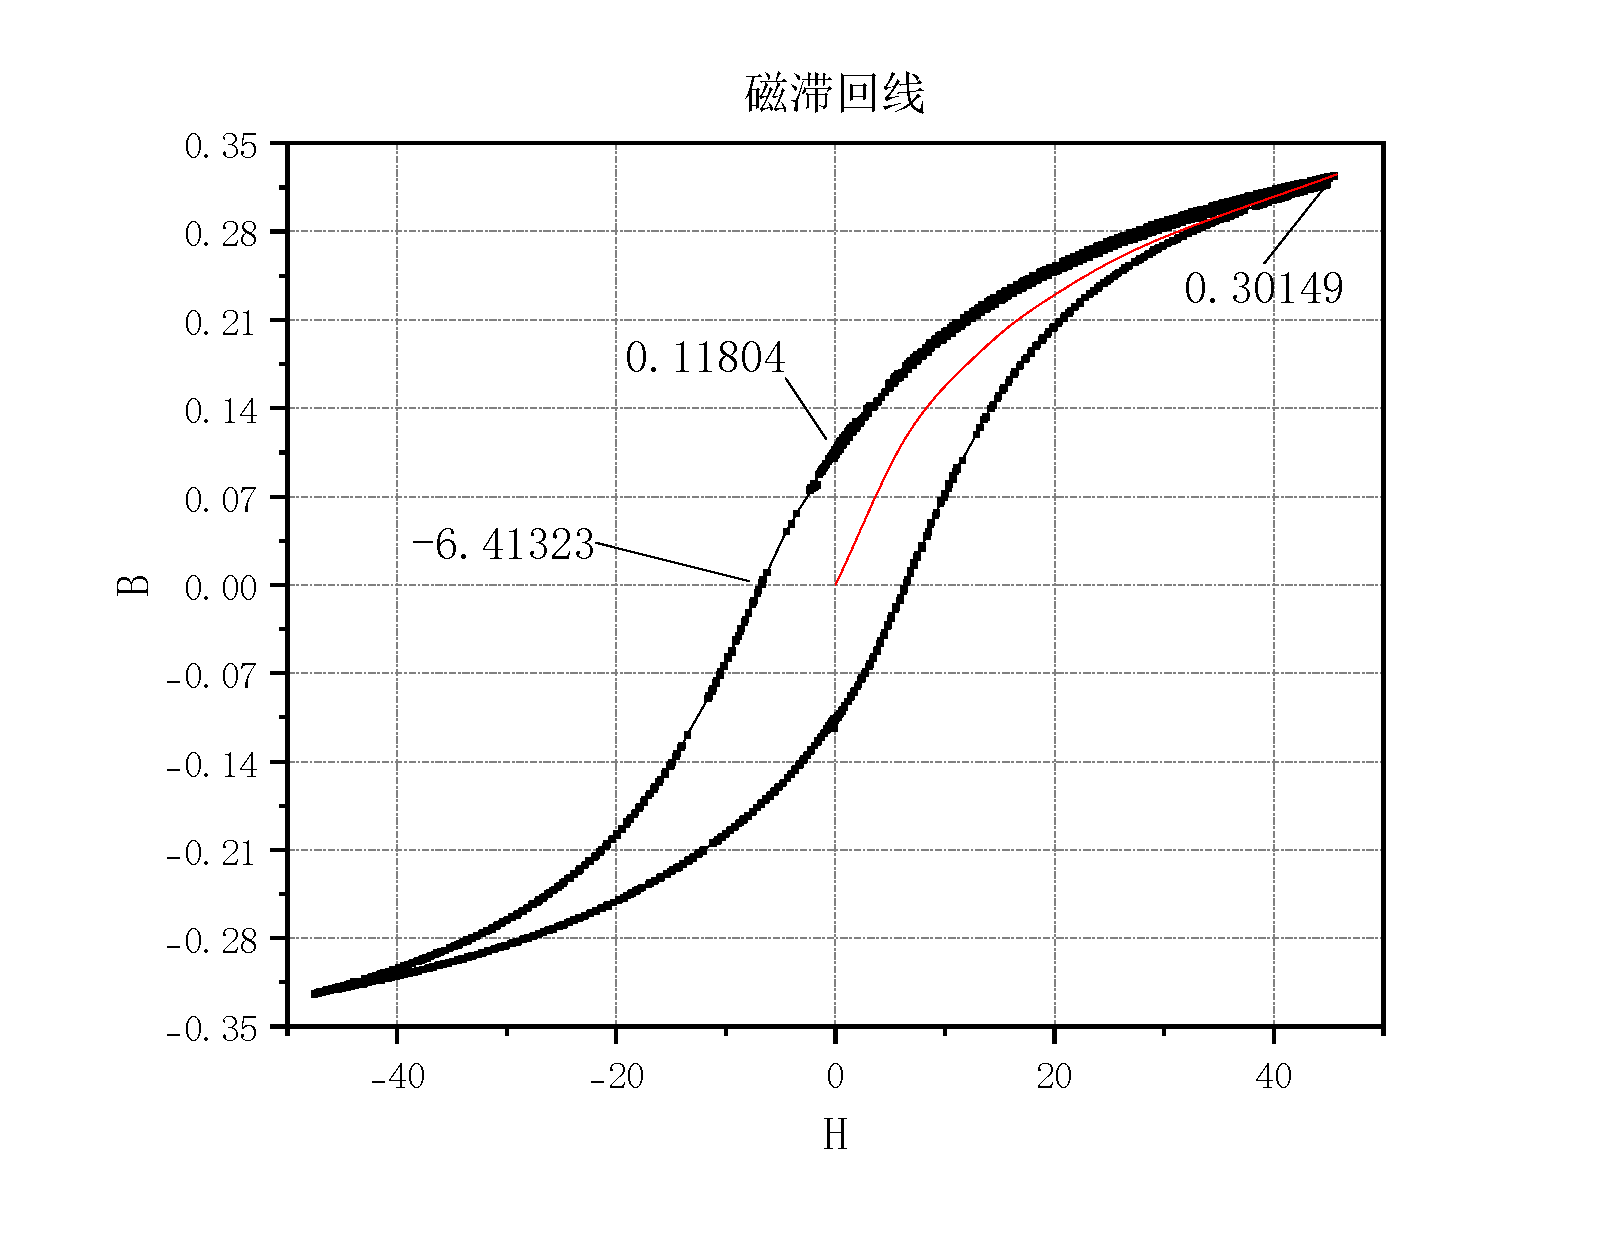
\includegraphics[width=0.8\textwidth]{fig3.pdf}}
        \end{figure}\par
        计算得到:
        \begin{table}[!ht]
            \centering\begin{tabular}{c c c}\hline
                样品 & 热导率 & 热容 \\ \hline
                \makebox[50mm]{有机玻璃} & $ 0.264 \unit{\TTR}$ &\makebox[50mm]{$1.78*10^3 \unit{\J\per\kg\per\K}$} \\
                黑橡胶 & $ 0.441 \unit{\TTR}$ & $1.62*10^3 \unit{\J\per\kg\per\K}$ \\\hline
            \end{tabular}
        \end{table}
\section{思考题}
    \begin{enumerate}
        \item 根据实测值和参考值估算这三种材料的热导率的相对误差,并分析误差的来源。(铝合金 $k=\qrange{121}{180}{\TTR}$ )\par
        取 121 \unit{\TTR} 为参考值,则相对误差为:0.36\% ,对于铝合金样品,误差可能有以下来源:
        \begin{itemize}
            \item 湿度可能会有略微影响
            \item 硅脂涂抹过多,硅脂导热并不好,仅用来填平空隙防止空气进入
            \item 仪器测量、稳态法方法导致的系统误差
        \end{itemize}
        \item 平板热流法实验使用铜—康铜热电偶测温。为什么冷端要放到冰水混合物中?\par
        因为实验时需测得热端温度,因此需要让冷端温度已知,才可以计算得到热端温度,但如果实验中仅仅只需要计算两个热端温差,可以参照准稳态法将两个冷端放在同一个保温杯中,保证温度相同即可。
        \item 比较稳态法和准稳态法测量材料热导率的优缺点\par
            稳态法:
            \begin{itemize}
                \item 数学表达式简单,但精度低
                \item 是低电导率样品的绝对和主要方法
                \item 部分适用于粉末状、颗粒状或固体形式
                \item 要求材料达到稳定热传导的状态的时间长
                \item 对于平板状和空心圆筒状样品,热量散失不可忽略;对于异形样品,很难测试
            \end{itemize}\par
            准稳态法:
            \begin{itemize}
                \item 测量时间更短,精度更高
                \item 测量范围宽
                \item 部分适用于粉末状、颗粒状或固体形式
                \item 要求材料达到稳定热传导的状态的时间长
                \item 对于平板状和空心圆筒状样品,热量散失不可忽略
            \end{itemize}
        \item 已知有机玻璃的热导率 $ \lambda = 0.17 ~\unit{\TTR}$ ,比热 $c = 1.31*10^3 ~\unit{\J\per\kg\per\K}$ ;橡胶的热导率 $ \lambda =0.426 ~\unit{\TTR}$ ,比热 $c=1.19*10^3 ~\unit{\J\per\kg\per\K}$ 。根据实测值和参考值估算两种材料的热导率和比热的相对误差,并分析误差的来源\par
            \begin{table}[!ht]
                \centering\begin{tabular}{c c c}\hline
                    样品 & 热导率相对误差 & 热容相对误差 \\ \hline
                    \makebox[50mm]{有机玻璃} & $ 55.34\% $ &\makebox[50mm]{$ 36.52\% $} \\
                    黑橡胶 & $ 3.53\% $ & $ 36.51\% $ \\\hline
                \end{tabular}
            \end{table}
            误差来源:
                \begin{itemize}
                    \item 可能没有拧紧转轮,导致样品对外有散热
                    \item 可能未等到仪器完全散热即开始下一组测试
                    \item 但与其它同学测得的结果较为接近,也有可能是长时间放置导致样品实际热学性能与标准产生偏差
                    \item 在实际操作实验过程中待测样品周围的空气温度并非一直不变,样品室内空气温度升高使得测量值较实际值偏大
                    \item 测试时并非在同一台机器,而是两台机器,仪器的不同也会造成误差
                \end{itemize}\par
        \item 判定系统达到准稳态导热的依据是什么?\par
        准稳态是指物质内各个点的温升速率相同且保持不变,样品内两点间温差恒定。也就是 $V_t$ 和 $\Delta V$不变
        \end{enumerate}
\end{document}